
\documentclass[10pt,letterpaper]{article}
\usepackage[top=0.85in,left=2.75in,footskip=0.75in]{geometry}

% amsmath and amssymb packages, useful for mathematical formulas and symbols
\usepackage{amsmath,amssymb}

% Use adjustwidth environment to exceed column width (see example table in text)
\usepackage{changepage}

% textcomp package and marvosym package for additional characters
\usepackage{textcomp,marvosym}

% cite package, to clean up citations in the main text. Do not remove.
\usepackage{cite}

% Use nameref to cite supporting information files (see Supporting Information section for more info)
\usepackage{nameref,hyperref}

% line numbers
\usepackage[right]{lineno}

% ligatures disabled
\usepackage[nopatch=eqnum]{microtype}
\DisableLigatures[f]{encoding = *, family = * }

% color can be used to apply background shading to table cells only
%\usepackage[table]{xcolor}

% array package and thick rules for tables
\usepackage{array}

% create "+" rule type for thick vertical lines
\newcolumntype{+}{!{\vrule width 2pt}}

% create \thickcline for thick horizontal lines of variable length
\newlength\savedwidth
\newcommand\thickcline[1]{%
  \noalign{\global\savedwidth\arrayrulewidth\global\arrayrulewidth 2pt}%
  \cline{#1}%
  \noalign{\vskip\arrayrulewidth}%
  \noalign{\global\arrayrulewidth\savedwidth}%
}

% \thickhline command for thick horizontal lines that span the table
\newcommand\thickhline{\noalign{\global\savedwidth\arrayrulewidth\global\arrayrulewidth 2pt}%
\hline
\noalign{\global\arrayrulewidth\savedwidth}}


% Remove comment for double spacing
%\usepackage{setspace} 
%\doublespacing

% Text layout
\raggedright
\setlength{\parindent}{0.5cm}
\textwidth 5.25in 
\textheight 8.75in

% Bold the 'Fig #' in the caption and separate it from the title/caption with a period
% Captions will be left justified
\usepackage[aboveskip=1pt,labelfont=bf,labelsep=period,justification=raggedright,singlelinecheck=off]{caption}
\renewcommand{\figurename}{Fig}

% Use the PLoS provided BiBTeX style
\bibliographystyle{plos2015}

% Remove brackets from numbering in List of References
\makeatletter
\renewcommand{\@biblabel}[1]{\quad#1.}
\makeatother



% Header and Footer with logo
\usepackage{lastpage,fancyhdr,graphicx}
\usepackage{epstopdf}
\usepackage{lmodern}
%\pagestyle{myheadings}
\pagestyle{fancy}
\fancyhf{}
%\setlength{\headheight}{27.023pt}
%\lhead{\includegraphics[width=2.0in]{PLOS-submission.eps}}
\rfoot{\thepage/\pageref{LastPage}}
\renewcommand{\headrulewidth}{0pt}
\renewcommand{\footrule}{\hrule height 2pt \vspace{2mm}}
\fancyheadoffset[L]{2.25in}
\fancyfootoffset[L]{2.25in}
\lfoot{\today}

%% Include all macros below

\newcommand{\lorem}{{\bf LOREM}}
\newcommand{\ipsum}{{\bf IPSUM}}

%% END MACROS SECTION

%% personal packages and macro
%%% packages
\usepackage[utf8]{inputenc}        % allow utf-8 input
\usepackage[T1]{fontenc}           % use 8-bit T1 fonts
\usepackage[dvipsnames, table]{xcolor}
\usepackage{tabularx}
\usepackage{multirow}
\usepackage{pifont}
\usepackage{csvsimple}
\usepackage[font={small},textfont={it},labelfont={bf}]{caption}
\usepackage{subcaption}
\usepackage{graphicx}
\usepackage{url}                   % simple URL typesetting
\usepackage{booktabs}              % professional-quality tables
\usepackage{makecell}
\usepackage{amsfonts}              % blackboard math symbols
\usepackage{amsmath}
\usepackage{nicefrac}              % compact symbols for 1/2, etc.
\usepackage{microtype}             % microtypography
\usepackage{enumitem}
\usepackage[export]{adjustbox}


%not compatible with cite package
%\usepackage[natbib=true,style=nature,maxnames=999,maxcitenames=2,backend=biber]{biblatex}
%\addbibresource{references.bib}

%%% macros
\DeclareMathOperator*{\argmin}{arg\,min}
\newcommand{\indep}{\perp \!\!\! \perp}
\newtheorem{assumption}{Assumption}

\definecolor{dark_blue}{rgb}{0,0,.65}
\definecolor{dark_green}{rgb}{0,.5,.15}

\hypersetup{pdftex,  % needed for pdflatex
  breaklinks=true,  % so long urls are correctly broken across lines
  colorlinks=true,
  linkcolor=dark_blue,
  citecolor=dark_green,
}
\colorlet{P}{ForestGreen}
\colorlet{I}{MidnightBlue}
\colorlet{C}{YellowOrange}
\colorlet{O}{DarkOrchid}
\colorlet{T}{Gray}



\begin{document}
\vspace*{0.2in}

\section*{Supporting information}


\paragraph*{S5 Appendix}
\label{apd:hyper_parameter_search}
{\bf Hyper-parameter search for the nuisance models.}

We followed a two-step procedure to train the nuisance models (eg. ($\hat e,
    \hat \mu$) for the AIPW causal estimator), taking inspiration from the
computationally cheap procedure from
\cite[section~3.3]{bouthillier2021accounting}. First, for each nuisance
model, we fit a random parameter search with 5-fold cross validation and 10
iterations on the full dataset. Each iteration fit a model with a random
combination of parameters in a predefined grid, then evaluate the
performance by cross-validation. The best hyper-parameters $\hat
    \lambda^{\star}$ are selected as the ones reaching the minimal score across
all iterations. Then, we feed this parameters to the causal estimator. The
single robust estimators (matching, IPW and TLearner) refit the
corresponding estimator only once on the full dataset, then estimate the
ATE. The doubly-robust estimators use a cross-fitting procedure (K=5) to fit
the nuisances then estimate the ATE. Fig
\ref{apd:fig:hyper_parameter_search} illustrates the procedure and Table
\ref{apd:table:hyper_parameter_search} details the hyper-parameters grid for
the random search.

\begin{figure}[!h]
    \begin{minipage}{.38\linewidth}
        \caption{{\bf Hyper-parameter search procedure.}}\label{apd:fig:hyper_parameter_search}
    \end{minipage}%
    \hfill
    \begin{minipage}{.6\linewidth}
        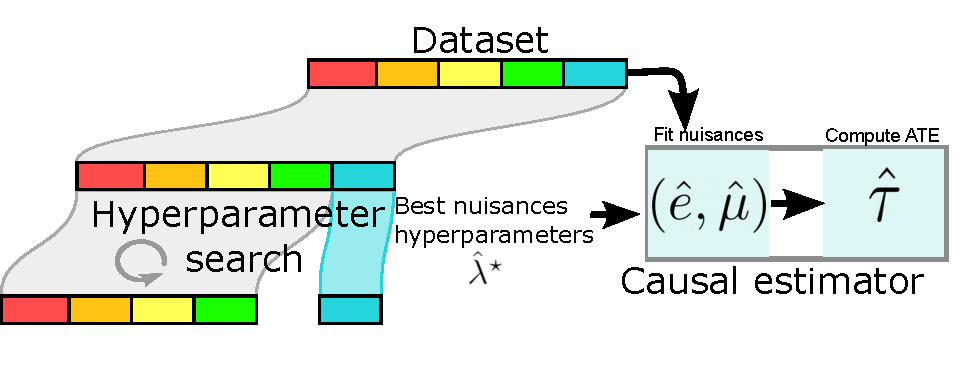
\includegraphics[width=\linewidth]{img_supp_final/hp_search_procedure.pdf}
    \end{minipage}%
\end{figure}

\begin{table}[!h]
    \resizebox{\textwidth}{!}{%
        \begin{tabular}{llll}
            \toprule
            {}             & estimator              & nuisance  & Grid                                                                       \\
            Estimator type &                        &           &                                                                            \\
            \midrule
            Linear         & LogisticRegression     & treatment & \{'C': logspace(-3, 2, 10)\}                                               \\
            Linear         & Ridge                  & outcome   & \{'alpha': logspace(-3, 2, 10)\}                                           \\
            Forest         & RandomForestClassifier & treatment & \{'n\_estimators': ['10', '100', '200'], 'max\_depth': ['3', '10', '50']\} \\
            Forest         & RandomForestRegressor  & outcome   & \{'n\_estimators': ['10', '100', '200'], 'max\_depth': ['3', '10', '50']\} \\
            \bottomrule
        \end{tabular}

    }\\
    \caption{\textbf{Hyper-parameter grid used during random search
            optimization.}}\label{apd:table:hyper_parameter_search}
\end{table}

\bibliography{references}


\end{document}
